\documentclass[11pt,a4paper]{article}
\usepackage[T2A]{fontenc}
\usepackage[utf8]{inputenc}
\usepackage[russian]{babel}
\usepackage[margin=19mm,headheight=15pt]{geometry}
\usepackage{amsmath,amssymb,booktabs,array,xcolor,enumitem,fancyhdr,graphicx,placeins}
\usepackage{xurl}
\usepackage[colorlinks=true,linkcolor=blue!50!black,urlcolor=blue!50!black]{hyperref}
\pdfstringdefDisableCommands{\def\hfill{ }}
\setlength{\parindent}{0pt}
\setlength{\parskip}{5pt}
\setlength{\emergencystretch}{3em}
\setlist[itemize]{leftmargin=*,topsep=3pt,itemsep=2pt,parsep=0pt}
\setlist[enumerate]{leftmargin=*,topsep=3pt,itemsep=2pt,parsep=0pt}
\pagestyle{fancy}\fancyhf{}
\fancyhead[L]{Сэмплирование: семинар 1}
\fancyhead[R]{Конспект преподавателя}
\fancyfoot[C]{\thepage}
\newcommand{\E}{\mathbb E}
\newcommand{\Pp}{\mathbb P}
\newcommand{\R}{\mathbb R}
\newcommand{\Normal}{\mathcal N}
\newcommand{\Var}{\operatorname{Var}}
\newcommand{\Cov}{\operatorname{Cov}}
\newcommand{\TV}{\operatorname{TV}}
\newcommand{\ESS}{\operatorname{ESS}}
\newcommand{\MCSE}{\operatorname{MCSE}}
\newcommand{\ind}{\mathbf 1}
\newcommand{\board}[1]{\par\emph{На доске.} #1\par}
\newcommand{\teach}[1]{\par\emph{Комментарий преподавателю.} #1\par}
% Match the normal-weight headings used in the recent Skoltech materials.
\makeatletter
\renewcommand\section{\@startsection{section}{1}{\z@}{-3.0ex \@plus -1ex \@minus -.2ex}{1.5ex \@plus .2ex}{\normalfont\Large}}
\renewcommand\subsection{\@startsection{subsection}{2}{\z@}{-2.5ex \@plus -.8ex \@minus -.2ex}{1.0ex \@plus .2ex}{\normalfont\large}}
\makeatother
\begin{document}
\begin{center}
{\LARGE Сэмплирование. Семинар 1}\\[5pt]
{\large Метод отклонений, марковские цепи, эргодичность\\
и алгоритм Гиббса}\\[5pt]
ИППИ РАН \textbar\ Байесовские методы машинного обучения \textbar\ Осень 2026
\end{center}

Цель занятия --- научиться строить выборку из распределения, известного с
точностью до нормировочной константы, и различать три утверждения:
распределение инвариантно для перехода; закон цепи приближается к нему;
среднее вдоль траектории приближается к нужному интегралу. Метод отклонений
даёт независимые принятые значения. Гиббс строит зависимую траекторию с
нужным инвариантным распределением; её полезность зависит от перемешивания.

Формат: 60 минут объяснения и выводов на доске, затем 30 минут демонстрации
заполненного \texttt{sampling\_first\_solutions.ipynb}. Время написания кода
студентами в этот маршрут не заложено. Метрополис, Метрополис--Гастингс,
его связь с Гиббсом и гамильтонова динамика относятся ко второму семинару.
Здесь условие детального равновесия вводится и применяется к Гиббсу.

\section*{Маршрут на 90 минут}
\begin{center}\small
\begin{tabular}{@{}p{15mm}p{47mm}p{99mm}@{}}
\toprule
Минуты & Блок & Что должно остаться на доске или экране\\
\midrule
0--6 & Постериор и интегралы & $\pi=\widetilde\pi/Z$; среднее Монте-Карло и ошибка iid.\\
6--18 & Метод отклонений & Глобальная огибающая; вывод закона принятого значения; $Z/M$.\\
18--33 & Марковская цепь & $\mu_{t+1}=\mu_tP$; $\pi P=\pi$; неприводимость и период.\\
33--42 & Детальное равновесие & Парные потоки; одна строка доказательства стационарности.\\
42--60 & Гиббс & Условные распределения, инвариантность, выбор координаты и полный проход.\\
\midrule
60--68 & Ноутбук: отклонения & Геометрия принятия, гистограмма и точные ориентиры.\\
68--75 & Ноутбук: цепи & Сходимость, периодичность, зависимость от старта.\\
75--90 & Ноутбук: Гиббс & Траектории, автокорреляции, цена сильной корреляции.\\
\bottomrule
\end{tabular}\end{center}

Предполагаются формула Байеса, условная вероятность, матричное умножение,
нормальная плотность и интеграл как ожидание. Все данные синтетические;
ноутбук выполняется на CPU без загрузки данных. Требуются NumPy, SciPy,
Matplotlib и IPython. Сохранённые выводы позволяют провести демонстрацию
без ожидания вычислений. Приложение с байесовской моделью находится за
пределами 90 минут.

\teach{Сохраните справа на доске три строки: $\pi P=\pi$;
$\mu_0P^t\to\pi$; $N^{-1}\sum_t f(X_t)\to\E_\pi f$.
Возвращайтесь к ним при каждом контрпримере. Если времени мало, сократите
обсуждение неравновесных потоков и численной оценки ESS; сохраните доказательство
метода отклонений, условия конечномерной теоремы и доказательство Гиббса.}

\section{Доска 1. Зачем нужны значения из постериора \hfill 0--6 минут}

Пусть $D$ --- наблюдения, $\theta$ --- параметр. Формула Байеса даёт
\[
 \pi(\theta)=p(\theta\mid D)
 =\frac{p(D\mid\theta)p(\theta)}{p(D)}
 =\frac{\widetilde\pi(\theta)}{Z},\qquad
 Z=\int\widetilde\pi(\theta)\,d\theta,\quad 0<Z<\infty.
\]
Вычислить числитель в заданной точке часто легче, чем интеграл.
Нас интересуют $I=\E_\pi f(\Theta)$: среднее параметра, вероятность события
($f=\ind_A$), ожидаемые потери или предсказание
\[
 p(y_*\mid x_*,D)=\E_{\pi(\theta)}p(y_*\mid x_*,\theta).
\]
Для независимых $\Theta_i\sim\pi$ оценка и её дисперсия равны
\[
 \widehat I_N=\frac1N\sum_{i=1}^N f(\Theta_i),\qquad
 \E\widehat I_N=I,\qquad
 \Var(\widehat I_N)=\frac{\Var_\pi f}{N}.
\]
При $\E_\pi|f|<\infty$ действует закон больших чисел; формуле дисперсии
нужен конечный второй момент. Для зависимых значений ковариации между
слагаемыми остаются и формула $\Var_\pi f/N$ обычно неверна.

\board{Написать $\Var(\sum_i f_i)=\sum_{i,j}\Cov(f_i,f_j)$.
Спросить, какой шаг использует независимость. Полный вывод ЦПТ сейчас не нужен.}

Разброс постериора описывает неопределённость параметра. Стандартная ошибка
Монте-Карло описывает точность вычисления конкретного интеграла. Увеличение
числа сэмплов уменьшает вторую величину, сохраняя сам постериор.

\section{Доска 2. Метод отклонений \hfill 6--18 минут}

\subsection{Конструкция и доказательство}
Выберем нормированную плотность $q$, из которой легко получать независимые
значения. Нужна известная конечная константа $M$ такая, что
\[
 \widetilde\pi(x)\le Mq(x)\quad\text{на всём носителе},\qquad
 q(x)>0\ \text{там, где}\ \widetilde\pi(x)>0.
\]
На каждом испытании независимо генерируем $X\sim q$ и $U\sim U(0,1)$.
Принимаем $X$, если
\[
 U\le\frac{\widetilde\pi(X)}{Mq(X)}.
\]
Иначе выбрасываем предложение и начинаем новое независимое испытание.
Нормировочная константа $Z$ в этом решении не участвует.

Обозначим принятие через $A$. Для любого измеримого множества $B$
\begin{align*}
 \Pp(X\in B,A)
 &=\int_B q(x)\frac{\widetilde\pi(x)}{Mq(x)}\,dx
 =\frac1M\int_B\widetilde\pi(x)\,dx,\\
 \Pp(A)&=\frac ZM,\\
 \Pp(X\in B\mid A)
 &=\frac{\int_B\widetilde\pi(x)\,dx/M}{Z/M}
 =\int_B\pi(x)\,dx.
\end{align*}
Последовательные принятые значения независимы и имеют закон $\pi$, потому
что каждое следующее получено из нового независимого блока испытаний.
Число предложений до одного принятия геометрическое со средним $M/Z$.
Для заранее заданных $N$ принятых значений ожидаемая цена --- $NM/Z$ испытаний.

\teach{Здесь $M$ ограничивает \emph{ненормированное} отношение
$\widetilde\pi/q$, поэтому может быть меньше 1. Вероятность принятия
равна $Z/M$. Формула $1/M$ относится к огибающей уже нормированной плотности.
Проверка огибающей только на сетке не доказывает глобальное неравенство.
Если отношение превышает 1, нельзя исправлять алгоритм обрезанием:
огибающая выбрана неверно.}

\subsection{Общий пример: монета}
Пусть $\theta\sim\operatorname{Beta}(2,2)$ и наблюдались один орёл и пять
решек. Для определённой последовательности наблюдений
\[
 p(D\mid\theta)\propto\theta(1-\theta)^5,\qquad
 \widetilde\pi(\theta)=\theta^2(1-\theta)^6\ind_{(0,1)}(\theta),
 \qquad \pi=\operatorname{Beta}(3,7).
\]
В нормировке ядра опущена константа prior. Поэтому
$Z=B(3,7)=1/252$ --- нормировочная константа выбранного ядра;
evidence указанной последовательности равен $6Z$.

Для $q=U(0,1)$ максимум найдём аналитически:
\[
 \frac{d}{d\theta}\log\widetilde\pi(\theta)
 =\frac2\theta-\frac6{1-\theta}=0
 \quad\Longrightarrow\quad\theta_*=\frac14,
 \qquad M=\left(\frac14\right)^2\left(\frac34\right)^6.
\]
Вторая производная отрицательна, на границах ядро равно нулю, значит это
глобальный максимум. Точные ориентиры для демонстрации:
\[
 Z=\frac1{252},\qquad \frac ZM\simeq0.3567,\qquad
 \E_\pi\theta=0.3,\quad \Var_\pi\theta=\frac{21}{1100},\quad
 \Pp_\pi(\theta>1/2)=\frac{23}{256}.
\]
Для равномерного $q$ рисуем точки $(X,MU)$ в прямоугольнике:
принимаются точки под графиком ядра. Площадь под графиком равна $Z$.

\begin{figure}[htbp]\centering
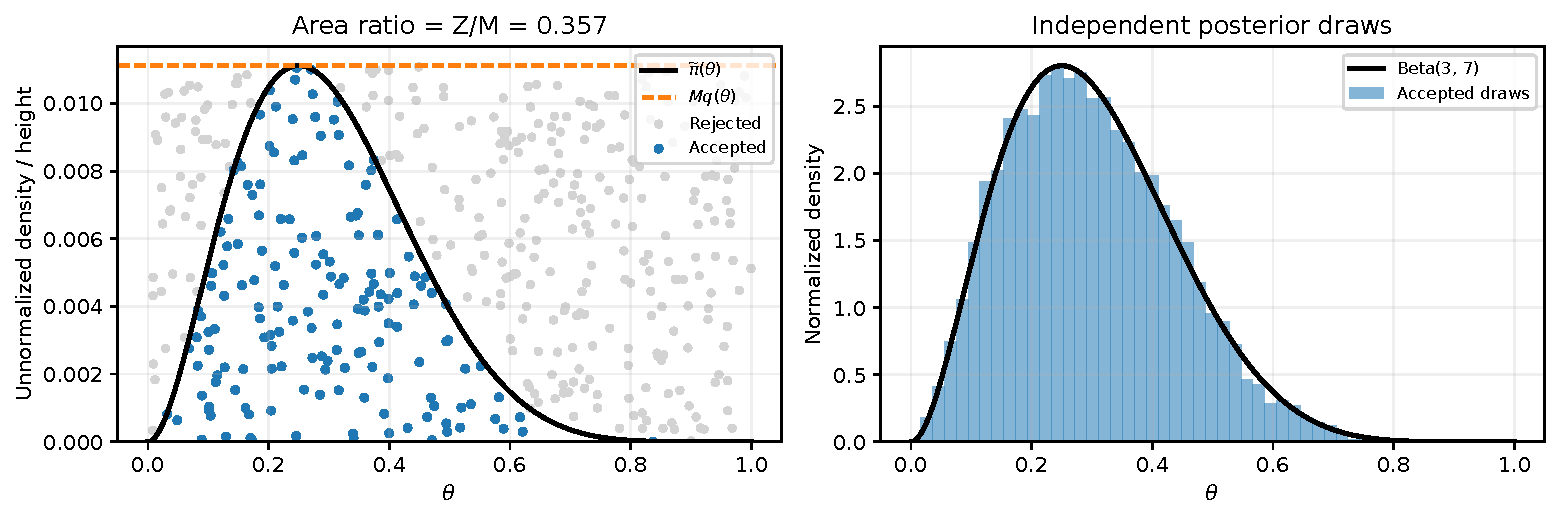
\includegraphics[width=.94\linewidth]{assets/rejection_geometry.pdf}
\caption{Метод отклонений для постериора монеты. Конкретные значения
эмпирических оценок находятся в выполненном ноутбуке.}
\end{figure}
\FloatBarrier

\board{Сначала доказать закон принятого значения, затем находить $M$.
Вопрос: меняется ли алгоритм при замене $\widetilde\pi$ на
$c\widetilde\pi$ и $M$ на $cM$? Нет: отношение принятия сохраняется.}

Метод ограничен качеством глобальной огибающей. Для произведения $d$
одинаковых целей и произведения предложений огибающая $M^d$ даёт
вероятность принятия $(Z/M)^d$. Даже хороший одномерный метод тогда
быстро становится дорогим. Это пример, а не теорема о любом выборе $q$.

\section{Доска 3. Марковская цепь и стационарность \hfill 18--26 минут}

Сначала рассмотрим конечное множество состояний $S=\{1,\ldots,m\}$.
Однородная марковская цепь удовлетворяет
\[
 \Pp(X_{t+1}=j\mid X_0,\ldots,X_t)
 =\Pp(X_{t+1}=j\mid X_t)=P_{X_tj}.
\]
Матрица перехода $P$ имеет неотрицательные элементы и суммы строк 1.
Распределения записываем \emph{строками}: если $\mu_t(j)=\Pp(X_t=j)$, то
\[
 \mu_{t+1}(j)=\sum_i\mu_t(i)P_{ij},\qquad
 \mu_{t+1}=\mu_tP,\qquad \mu_t=\mu_0P^t.
\]
Величина $(P^t)_{ij}$ --- вероятность попасть из $i$ в $j$ за $t$ шагов.

Распределение $\pi$ называется стационарным, или инвариантным, если
\[
 \pi P=\pi,\qquad \pi_j\ge0,\qquad\sum_j\pi_j=1.
\]
Если $X_0\sim\pi$, то $X_t\sim\pi$ при любом $t$, но соседние состояния
обычно зависимы. Это утверждение само по себе ничего не говорит о старте
из фиксированного состояния и не обеспечивает единственность $\pi$.

Пример для ноутбука:
\[
 \pi=(0.2,0.5,0.3),\qquad
 P=\begin{pmatrix}
 .5&.3&.2\\ .12&.70&.18\\ 2/15&.3&17/30
 \end{pmatrix}.
\]
Проверяем суммы строк и $\pi P=\pi$. Из любого состояния можно попасть
в любое за один шаг; положительная диагональ допускает ожидание.
Итерации $\mu_0P^t$ --- точные законы, а не одна случайная траектория.

\board{Умножить строку $\pi$ на матрицу хотя бы для одной координаты.
Обязательно подписать направление: $P_{ij}$ означает $i\to j$.}

\section{Доска 4. Эргодичность и два контрпримера \hfill 26--33 минуты}

Цепь неприводима, если для любых $i,j$ существует $n\ge0$, при котором
$(P^n)_{ij}>0$. Период состояния
\[
 d(i)=\gcd\{n\ge1:(P^n)_{ii}>0\}.
\]
В неприводимой цепи периоды всех состояний совпадают. Цепь апериодична,
если этот период равен 1. Положительная вероятность остаться в одном
состоянии достаточна для апериодичности \emph{неприводимой} цепи.

Теорема для \emph{конечного} $S$. Неприводимость обеспечивает единственное
стационарное распределение $\pi$ с положительными компонентами. Если
дополнительно выполнена апериодичность, то для любого начального закона
\[
 \|\mu_0P^t-\pi\|_{\TV}
 =\frac12\sum_j|\mu_0P^t(j)-\pi_j|\longrightarrow0.
\]
Такую конечную цепь в этом семинаре называем эргодической. Для счётного
бесконечного пространства нужна положительная возвратность; для
непрерывного пространства формулировки используют неприводимость и
возвратность относительно меры. Конечную теорему нельзя автоматически
применять к непрерывному Гиббсу.

Закон больших чисел для неприводимой конечной цепи утверждает, что
для любой функции $f:S\to\R$ и любого старта
\[
 \frac1N\sum_{t=1}^N f(X_t)\longrightarrow
 \sum_j\pi_j f(j)\quad\text{почти наверное}.
\]
Здесь апериодичность не требуется. Сходимость законов в отдельный момент
и сходимость средних вдоль траектории --- разные результаты.

\begin{center}\small
\begin{tabular}{@{}p{34mm}p{57mm}p{70mm}@{}}
\toprule
Пример & Что верно & Что ломается\\
\midrule
$P=\left(\begin{smallmatrix}0&1\\1&0\end{smallmatrix}\right)$ &
Неприводима, $\pi=(1/2,1/2)$ единственна; доля посещений стремится к $1/2$. &
Период 2; закон из фиксированного старта чередуется и не сходится.\\[4pt]
$P=I_2$ & Любое распределение стационарно. &
Цепь приводима; траектория навсегда остаётся в начальной точке.\\
\bottomrule
\end{tabular}\end{center}

\teach{Не выводите скорость сходимости из одного условия существования
предела. Неприводимая апериодическая цепь тоже может очень медленно
перемешиваться. Длинная траектория в одной области не доказывает, что
остальных областей нет.}

\section{Доска 5. Условие детального равновесия \hfill 33--42 минуты}

Для заданной положительной $\pi$ условие имеет вид
\[
 \boxed{\pi_iP_{ij}=\pi_jP_{ji}\quad\text{для всех }i,j.}
\]
В стационарном режиме $\pi_iP_{ij}$ --- вероятность пары $(X_t=i,X_{t+1}=j)$.
Детальное равновесие означает равенство встречных потоков для каждой пары.
Просуммировав по $i$, получаем стационарность:
\[
 (\pi P)_j=\sum_i\pi_iP_{ij}
 =\sum_i\pi_jP_{ji}=\pi_j\underbrace{\sum_iP_{ji}}_{1}=\pi_j.
\]
В последней сумме индекс $j$ фиксирован: это сумма \emph{строки} $j$.
Детальное равновесие --- достаточное условие стационарности. Для
стационарной цепи оно также задаёт обратимость во времени.

В трёхсостоянийном примере встречные потоки равны $0.06$, $0.04$ и $0.09$:
\[
 \operatorname{diag}(\pi)P=
 \begin{pmatrix}.10&.06&.04\\.06&.35&.09\\.04&.09&.17\end{pmatrix}.
\]
Вычислить эту матрицу в ноутбуке полезнее, чем просто проверить
стационарность: видны попарные ограничения.

\subsection{Что условие не гарантирует}
$P=I$ удовлетворяет детальному равновесию относительно любой $\pi$, но не
обеспечивает нужного исследования пространства. Периодическое переключение
двух состояний также обратимо. Поэтому отдельно проверяем неприводимость
и апериодичность.

Детальное равновесие не необходимо для стационарности. Возьмём
\[
 P_{\circlearrowright}=\frac12I_3+\frac12
 \begin{pmatrix}0&1&0\\0&0&1\\1&0&0\end{pmatrix},\qquad
 \pi=(1/3,1/3,1/3).
\]
Суммы столбцов равны 1, следовательно $\pi P_{\circlearrowright}=\pi$.
Но $\pi_1P_{12}=1/6$, а $\pi_2P_{21}=0$. Цепь неприводима и апериодична,
несмотря на необратимость.

\board{Попросить сформулировать две независимые проверки для MCMC:
правильный инвариантный закон и возможность приближаться к нему из
используемых стартов. Доказательство детального равновесия решает первую
задачу, но не вторую.}

\section{Доска 6. Алгоритм Гиббса \hfill 42--54 минуты}

Пусть $x=(x_1,\ldots,x_d)$ и задана совместная плотность
$\pi(x)=\widetilde\pi(x)/Z$. Обозначим через $x_{-j}$ все координаты,
кроме $j$. Полное условное распределение
\[
 \pi(x_j\mid x_{-j})=
 \frac{\widetilde\pi(x_j,x_{-j})}
 {\int\widetilde\pi(u,x_{-j})\,du}
\]
не содержит глобального $Z$. Но сам одномерный условный закон должен
быть известен и доступен для сэмплирования. Гиббс не обещает, что это
всегда легко.

Один координатный шаг $K_j$ сохраняет $x_{-j}$ и генерирует
$x'_j\sim\pi(\cdot\mid x_{-j})$. Почему сохраняется совместное распределение?
Если вход имеет закон $\pi$, то
\[
 X_{-j}\sim\pi_{-j},\qquad
 X'_j\mid X_{-j}\sim\pi(\cdot\mid X_{-j})
 \quad\Longrightarrow\quad
 (X'_j,X_{-j})\sim\pi.
\]
Это восстановление совместного закона из маргинального и условного.

Можно увидеть и детальное равновесие. Для двух состояний с общими
$x_{-j}=y_{-j}=z$ плотность встречных потоков равна
\[
 \pi_{-j}(z)\pi(x_j\mid z)\pi(y_j\mid z),
\]
что симметрично по $x_j,y_j$. Между состояниями с разными оставшимися
координатами переход $K_j$ невозможен в обе стороны. Сам $K_j$ обычно
неприводим: он меняет лишь одну координату.

\subsection{Два варианта обхода координат}
Случайный выбор координаты: на каждом шаге независимо выбираем $J=j$
с фиксированной вероятностью $w_j>0$, $\sum_jw_j=1$, и применяем $K_j$.
Ядро $K=\sum_jw_jK_j$ сохраняет $\pi$ и обратимо: детальное равновесие
сохраняется при такой смеси. Если выбор зависит от текущего состояния,
это доказательство уже не работает автоматически.

Последовательный обход: применяем $K_1$, затем $K_2$, $\ldots$, $K_d$.
Один полный проход имеет ядро $K_{\rm sweep}=K_1K_2\cdots K_d$ и
\[
 \pi K_{\rm sweep}=(((\pi K_1)K_2)\cdots)K_d=\pi.
\]
Композиция инвариантных шагов инвариантна, но в общем случае необратима.
В ноутбуке одна итерация и одно сохранённое состояние --- полный проход.
Если записывать каждый подшаг детерминированного обхода, переход зависит
от фазы; для однородной цепи нужно учитывать фазу или наблюдать полные проходы.

Для двух координат реализация использует \emph{свежее} первое значение:
\[
 x^{(t+1)}\sim\pi(x\mid y^{(t)}),\qquad
 y^{(t+1)}\sim\pi(y\mid x^{(t+1)}).
\]
Одновременное независимое обновление обеих координат из условных законов
при старом состоянии, вообще говоря, не является этим алгоритмом и не
обязано сохранять $\pi$.

\teach{Корректные условные шаги ещё не дают автоматической гарантии
сходимости. Например, если масса лежит лишь на $(0,0)$ и $(1,1)$, каждое
полное условное распределение вырождено, а покоординатный Гиббс застревает.
Блоковое обновление обеих координат может устранить эту конкретную проблему.}

\section{Доска 7. Гауссовский пример \hfill 54--60 минут}

Пусть
\[
 \begin{pmatrix}X\\Y\end{pmatrix}\sim
 \Normal\!\left(\begin{pmatrix}0\\0\end{pmatrix},
 \begin{pmatrix}1&\rho\\\rho&1\end{pmatrix}\right),\qquad |\rho|<1.
\]
Его ненормированная плотность
\[
 \widetilde\pi(x,y)=\exp\left[-\frac{x^2-2\rho xy+y^2}{2(1-\rho^2)}\right].
\]
Дополняем квадрат по $x$:
\[
 x^2-2\rho xy+y^2=(x-\rho y)^2+(1-\rho^2)y^2.
\]
При фиксированном $y$ второе слагаемое входит в нормировку. Поэтому
\[
 X\mid Y=y\sim\Normal(\rho y,1-\rho^2),\qquad
 Y\mid X=x\sim\Normal(\rho x,1-\rho^2).
\]
Для независимых стандартных нормальных $\varepsilon_t,\eta_t$
\begin{align*}
 x_{t+1}&=\rho y_t+\sqrt{1-\rho^2}\,\varepsilon_{t+1},\\
 y_{t+1}&=\rho x_{t+1}+\sqrt{1-\rho^2}\,\eta_{t+1}.
\end{align*}
Условные средние вдоль координат тянут к наклонному гребню; при $\rho$
около 1 условная дисперсия мала, и траектория продвигается по нему медленно.
При $|\rho|<1$ переход полного прохода имеет строго положительную плотность
на $\R^2$; приведённая ниже AR(1)-форма даёт явную сходимость в этом примере.
При $|\rho|=1$ совместный закон вырожден, эти формулы плотности неприменимы.

\board{За последние шесть минут вывести условные распределения и написать
два обновления. Формулу автокорреляции ниже вывести уже во время
ноутбучной демонстрации, когда на экране видна медленная траектория.}

\begin{figure}[htbp]\centering
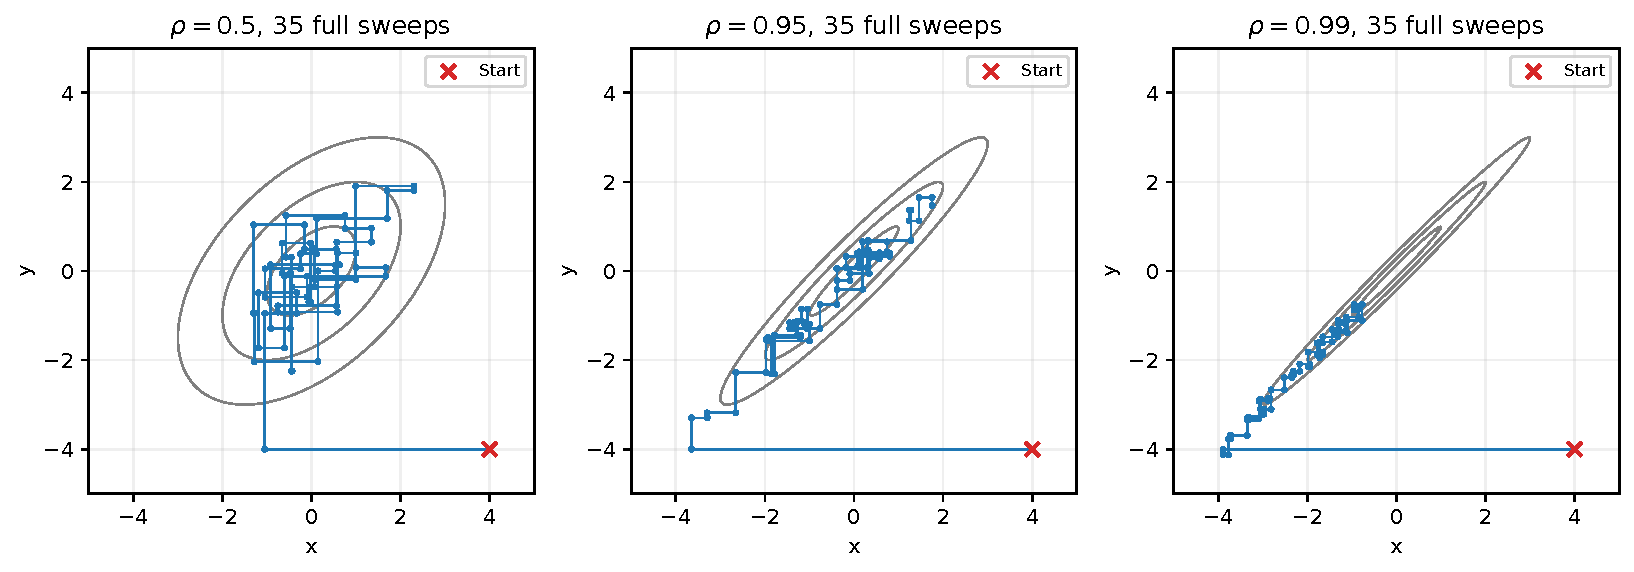
\includegraphics[width=.96\linewidth]{assets/gibbs_geometry.pdf}
\caption{Гиббс для коррелированной нормальной цели. Подшаги меняют одну
координату, а основной массив результатов хранит состояния после полного прохода.}
\end{figure}
\FloatBarrier

\section{Демонстрация в ноутбуке \hfill 60--90 минут}

Ноутбук полностью заполнен: определения, реализации, проверки, рисунки,
таблицы и ответы для обсуждения уже выполнены. Открыть его перед занятием,
перезапустить ядро и выполнить все ячейки. В классе проходить только три
основных блока; приложение не включать в тайминг.

\subsection{60--68. Независимые значения из постериора монеты}
Показать огибающую и принятые точки, затем гистограмму значений и точную
$\operatorname{Beta}(3,7)$. Сопоставить эмпирическую долю принятия с $Z/M$,
среднее с $0.3$, хвостовую вероятность с $23/256$. Основное внимание ---
почему принимаем именно такое отношение, а не на устройство графического кода.

Если запрашивается фиксированное число принятых значений, количество
предложений случайно. Для демонстрации доли принятия удобен отдельный
фиксированный бюджет испытаний: отношение принятого количества к бюджету
тогда непосредственно оценивает $Z/M$. Отбрасывание части уже вычисленного
последнего пакета должно быть явно учтено при сообщении цены.

Вопрос: одинаковы ли стандартное отклонение $\theta$ и стандартная ошибка
среднего? Ответ: первое около $0.1382$, второе для iid-выборки размера $N$
равно примерно $0.1382/\sqrt N$.

Вопрос: нужно ли знать $Z$ для алгоритма? Ответ: нет. Здесь $Z$ известна
для проверки и расчёта теоретической эффективности.

\subsection{68--75. Стационарность, сходимость законов и частоты}
Для трёх состояний показать $\mu_0P^t$ из разных стартов и расстояние до
$\pi$. Отдельно показать периодическое переключение двух состояний и
приводимый пример. Важно сравнить \emph{закон в момент $t$} с
\emph{долями посещений за время $1,\ldots,t$}.

\begin{figure}[htbp]\centering
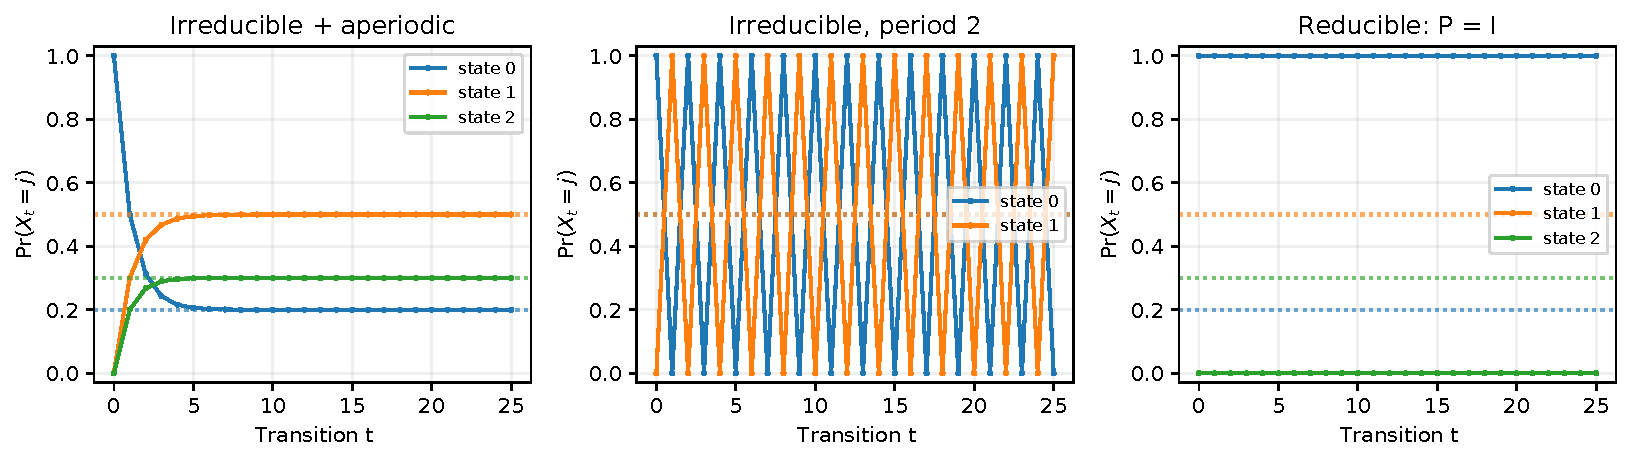
\includegraphics[width=.96\linewidth]{assets/markov_convergence.pdf}
\caption{Правильный инвариантный закон и приближение к нему из заданного
старта --- разные проверки. Периодическая цепь позволяет увидеть различие
между законом в отдельный момент и средними по времени.}
\end{figure}
\FloatBarrier

Вопрос: можно ли объявить цепь хорошей по проверке $\pi P=\pi$?
Ответ: этого мало; $P=I$ проходит такую проверку для любого $\pi$.
Вопрос: нужна ли обратимость любой работающей MCMC-цепи?
Ответ: нет; ленивый направленный цикл даёт явный контрпример.

\subsection{75--90. Геометрия и скорость Гиббса}
Показать условные распределения в коде и ступенчатый путь, затем сравнить
$\rho=0.5,0.95,0.99$ при одинаковом числе полных проходов. Сопоставить
траекторию на фоне точных контуров, значения одной координаты, накопленное среднее
и автокорреляцию. Одной гистограммы для оценки перемешивания недостаточно.

Подстановка первого обновления во второе даёт
\[
 y_{t+1}=\rho^2y_t+
 \sqrt{1-\rho^2}(\rho\varepsilon_{t+1}+\eta_{t+1}).
\]
Это AR(1) с коэффициентом $a=\rho^2$, независимыми гауссовскими инновациями
дисперсии $1-\rho^4$ и стационарной дисперсией 1. При произвольном
детерминированном $y_0$
\[
 \E y_t=a^t y_0,\qquad \Var(y_t)=1-a^{2t}.
\]
Следовательно, начальное смещение забывается, но при $a$ около 1 медленно.
В стационарном режиме для $f(x,y)=y$
\[
 r_f(k)=\rho^{2k},\qquad
 \tau_f=1+2\sum_{k=1}^{\infty}r_f(k)
 =\frac{1+\rho^2}{1-\rho^2},\qquad
 \ESS_f\simeq\frac N{\tau_f}.
\]
Здесь $N$ измеряется в полных проходах. Значения $\tau_f$ равны примерно
$1.67$, $19.51$ и $99.50$ для трёх выбранных $\rho$. Это точная
асимптотическая характеристика функции $f=y$, а не универсальное свойство
всех статистик цепи. При $\rho=0.99$ десять тысяч проходов дают для среднего
$y$ примерно столько же точности, сколько сто независимых значений.

\begin{figure}[htbp]\centering
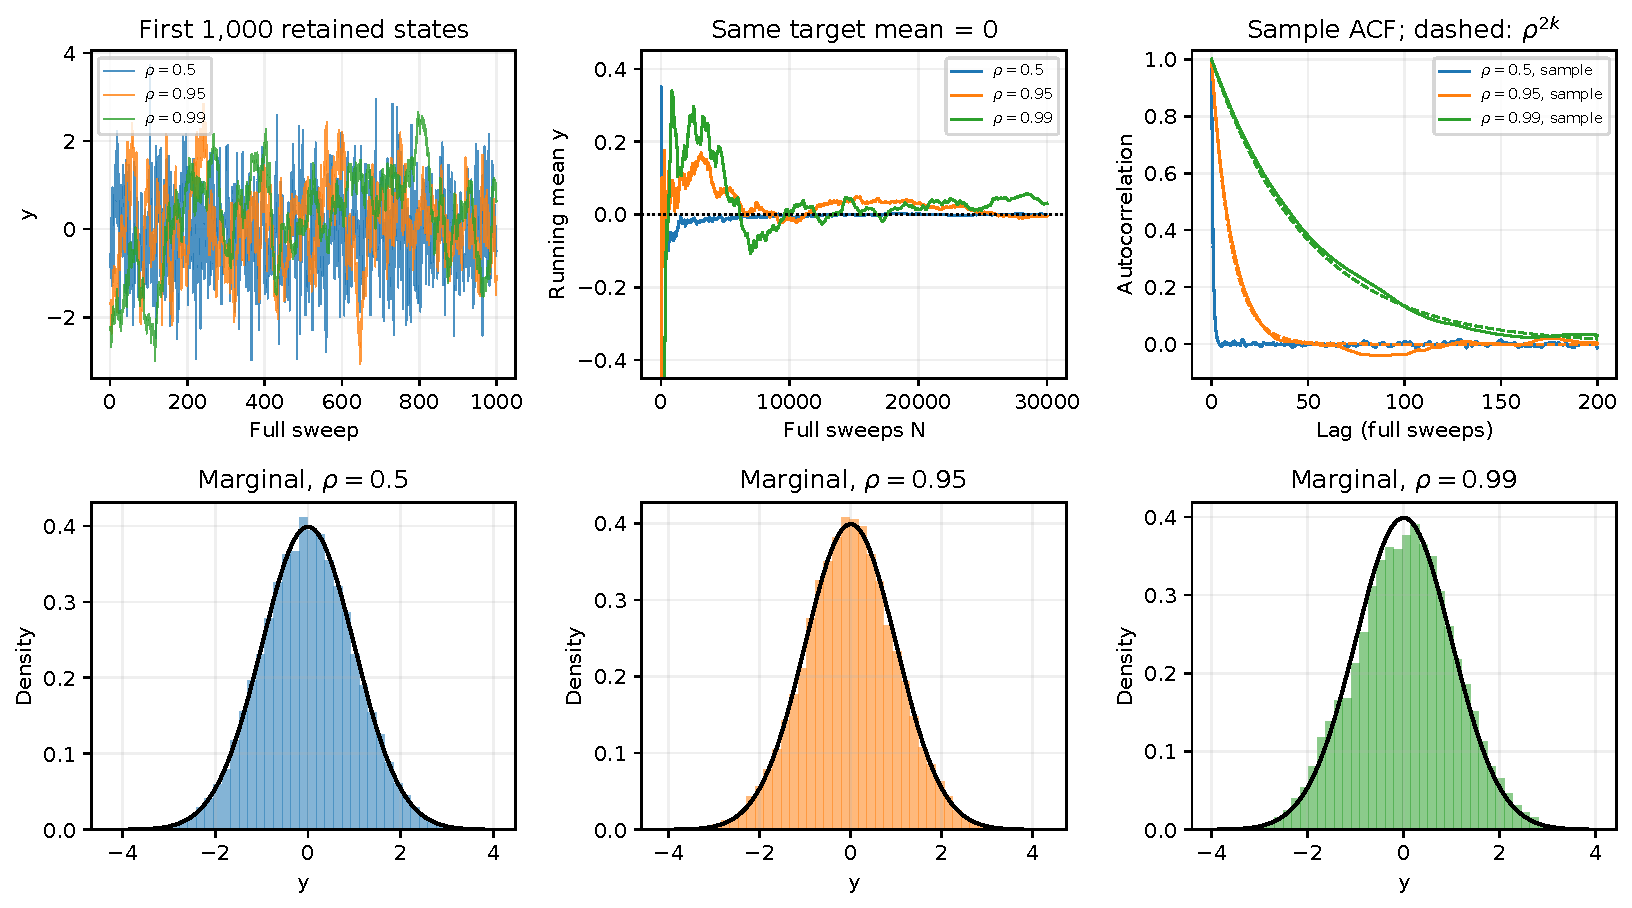
\includegraphics[width=.98\linewidth]{assets/gibbs_diagnostics.pdf}
\caption{Диагностика для одной функции вдоль цепи: траектория, среднее,
автокорреляция и сравнение с известной аналитической скоростью.}
\end{figure}
\FloatBarrier

В стационарном режиме точная формула дисперсии среднего при конечном $N$
имеет вид
\[
 \Var(\bar f_N)=\frac{\Var_\pi f}{N}
 \left[1+2\sum_{k=1}^{N-1}\left(1-\frac{k}{N}\right)r_f(k)\right].
\]
Если корреляции суммируемы и применима соответствующая ЦПТ для цепи,
асимптотическая стандартная ошибка равна
$\sqrt{\Var_\pi(f)\tau_f/N}$.
Для нашего гауссовского примера эти условия выполнены. Общая
эргодичность сама по себе не даёт ЦПТ с конечной дисперсией.

\teach{Эмпирическая ACF и любая оценка ESS шумят; длинные лаги особенно
ненадёжны. В ноутбуке аналитическая линия служит ориентиром. Оценку по
пакетным средним следует считать диагностикой: если в пакете мало
корреляционных длин, она может занижать ошибку. Не превращайте совпадение
случайного среднего с точным значением в тест корректности алгоритма.}

Burn-in уменьшает влияние старта, но не устраняет корреляцию оставшихся
значений. При точном стационарном старте burn-in не нужен. При произвольном
старте короткая выборка может быть смещена. Прореживание уменьшает
объём хранения, однако выбрасывание уже полученных значений обычно не
повышает точность на единицу выполненных переходов. В основном опыте
ноутбука начальное состояние получено из точной цели: burn-in не нужен,
сохраняются все проходы. Отдельный опыт показывает забывание разных
детерминированных стартов; в байесовском приложении используется burn-in.

\subsection{Заключительные вопросы на последнюю минуту}
\begin{enumerate}
\item Что дают принятые значения метода отклонений? Независимые значения
из цели при корректной глобальной огибающей.
\item Что доказывает детальное равновесие? Инвариантность заданного закона;
сходимость требует дополнительных свойств перехода.
\item Почему Гиббс работает без глобального $Z$? Эта константа сокращается
в полном условном распределении.
\item Почему правильные условные распределения могут давать медленный
метод? Переходы малы вдоль сильной зависимости или не соединяют компоненты носителя.
\item Что будет на следующем семинаре? Построение переходов, когда
непосредственно сэмплировать полные условные законы трудно.
\end{enumerate}

\appendix
\section{Дополнительные пояснения преподавателю}

\subsection{Почему полный проход Гиббса может быть необратим}
У координатного ядра оператор, обратный во времени, совпадает с ним самим.
У произведения таких операторов обратный порядок --- $K_d\cdots K_1$.
Произведение совпадёт с обратным только при дополнительных условиях.
Для стационарного гауссовского Гиббса с обходом $x$, затем $y$
\[
 \Cov(Y_t,X_{t+1})=\rho,\qquad
 \Cov(X_t,Y_{t+1})=\rho^3.
\]
При $0<|\rho|<1$ они различны, поэтому закон пары последовательных
состояний не инвариантен к перестановке времён. Само целевое
распределение при этом инвариантно. Этого вычисления в основном маршруте
не требуется.

\subsection{Почему нельзя обновлять обе координаты по старым значениям}
Предположим, что из стационарного состояния выполняют одновременно
$X'=\rho Y+\sqrt{1-\rho^2}\varepsilon$ и
$Y'=\rho X+\sqrt{1-\rho^2}\eta$ с независимыми шумами.
Тогда $\Cov(X',Y')=\rho^2\Cov(Y,X)=\rho^3$ вместо $\rho$.
Значит, такое параллельное обновление не сохраняет нужную корреляцию.
Это компактная аналитическая проверка важной ошибки реализации.

\subsection{Байесовская модель для необязательного продолжения}
Гауссовская двумерная цель выбрана для точной проверки геометрии.
Гиббс также естественно возникает в модели неизвестных среднего $\mu$
и точности $\lambda$ наблюдений:
\[
 z_i\mid\mu,\lambda\sim\Normal(\mu,\lambda^{-1}),\quad
 \mu\mid\lambda\sim\Normal(m_0,(\kappa_0\lambda)^{-1}),\quad
 \lambda\sim\operatorname{Gamma}(a_0,b_0).
\]
Используется параметризация Gamma через shape и \emph{rate}:
$p(\lambda)\propto\lambda^{a_0-1}e^{-b_0\lambda}$.
В NumPy аргумент \texttt{scale} равен $1/\texttt{rate}$.
Положим $n=|z|$, $\bar z=n^{-1}\sum_i z_i$, $S=\sum_i(z_i-\bar z)^2$.
Из совместного закона получаем, обозначив
\[
 \kappa_n=\kappa_0+n,\qquad
 m_n=\frac{\kappa_0m_0+n\bar z}{\kappa_n},
\]
полные условные распределения
\begin{align*}
 \mu\mid\lambda,z
 &\sim\Normal\!\left(m_n,\frac1{\kappa_n\lambda}\right),\\
 \lambda\mid\mu,z
 &\sim\operatorname{Gamma}\!\left(a_0+\frac{n+1}{2},\,
 b_0+\frac12\left[\sum_i(z_i-\mu)^2+\kappa_0(\mu-m_0)^2\right]\right).
\end{align*}
Добавка $1/2$ в shape второго условного закона возникает из нормирующего
множителя $\lambda^{1/2}$ условного prior для $\mu$. Это именно полный
условный закон, в котором $\mu$ фиксировано.

После интегрирования по $\mu$ маргинальный постериор имеет другие параметры:
\[
 \lambda\mid z\sim\operatorname{Gamma}(a_n,b_n),\quad
 a_n=a_0+\frac n2,\quad
 b_n=b_0+\frac S2+
 \frac{\kappa_0n(\bar z-m_0)^2}{2\kappa_n}.
\]
Поэтому точные контрольные значения:
$\E[\mu\mid z]=m_n$, $\E[\lambda\mid z]=a_n/b_n$,
$\Var(\mu\mid z)=b_n/[\kappa_n(a_n-1)]$ при $a_n>1$.
При необходимости можно получать независимые совместные значения
сначала из маргинального Gamma-постериора, затем из $\mu\mid\lambda,z$.
Для этого сопряжённого примера Гиббс полезен как учебная конструкция,
а прямое сэмплирование служит эталоном.

\section{Источники и связь с материалами курса}

Оформление и структура продолжают конспект ИППИ про EM и гауссовские
смеси: явная модель, вывод, проверяемая реализация, контролируемые
синтетические опыты и вопросы к интерпретации. Из материалов Skoltech
про sampling заимствован общий проверяемый постериор монеты
$\operatorname{Beta}(3,7)$. Содержание здесь переразбито под два семинара:
importance sampling и Метрополис--Гастингс в первый не входят.

\begin{enumerate}
\item K. Sigman (2007). \emph{Acceptance--Rejection Method}.
Страницы 1--2: доказательство метода; страница 4: пример Beta-распределения.
\url{https://www.columbia.edu/~ks20/4703-Sigman/4703-07-Notes-ARM.pdf}.
\item R. Weber. \emph{Markov Chains}, Cambridge course notes.
Разделы 9--11: сходимость законов, эргодические средние и детальное равновесие.
В теореме 10.2 отдельно отмечено, что для средних апериодичность не нужна.
\url{https://www.statslab.cam.ac.uk/~rrw1/markov/M.pdf}.
\item C. Geyer (2020). \emph{Stat 8501: Markov Chains}.
Раздел 5.4: условные обновления и варианты обхода Гиббса;
раздел 5.9: оценка ошибки Монте-Карло.
\url{https://www.stat.umn.edu/geyer/8501/markov.pdf}.
\item B. He, C. De Sa, I. Mitliagkas, C. R\'e (2016).
\emph{Scan Order in Gibbs Sampling: Models in Which It Matters and Bounds
on How Much}. NeurIPS. Разделы 2 и 5: случайный и последовательный обход,
необратимость полного прохода. Дополнительное чтение для преподавателя.
\url{https://pmc.ncbi.nlm.nih.gov/articles/PMC5361064/}.
\end{enumerate}

\end{document}
